\documentclass[10pt]{article}

\def\Type{LessonCaelan}
\def\TypeNum{Lesson 22}
\def\TypeTitle{Expectation and Variance}
\def\Semester{Fall 2021} %Not Used 
\def\Course{MATH 1190 \& 1210}

\usepackage{preambleDJ}
\usepackage{xcolor}

\begin{document}

\thispagestyle{firstpage}
\pagestyle{otherpages}
\vs{0.4}

\textbf{Intended Learning Outcomes}
After this lesson, you will be able to 

\begin{itemize}
    \item Define and explain the meaning of expectation and variance. (\target{P1, P2})
    \item Find the expectation and variance of a discrete random variable. (\target{P1})
    \item Find the expectation and variance of a continuous random variable. (\target{P2})
\end{itemize}

\vspace{-0.5cm}

\hrulefill

In this lesson, we will explore two key measures used to describe the characteristics of random variables: the expectation (mean) and variance. Expectation measures the "average" or "expected" value of a random variable, while variance measures how much the values of the random variable deviates from this average.

\begin{center}
({\it Expectation \& Variance of Discrete Random Variables})
\end{center}

\,\hfill\fbox{$\mu=E[X] = \displaystyle\sum_{x\in S_X} x\cdot p(x)$} \hfill\,

\,\hfill \fbox{$Var(X) = E[X^2]-\mu^2= \displaystyle\left(\sum_{x\in S_X} x^2\cdot p(x)\right)-\mu^2$}\hfill\,
Note: You might see elsewhere that the official definition of variance is $Var(X)=\displaystyle\sum_{x\in S_X}(x-\mu)^2p(x)$. The formula boxed above is different from but equivalent to the definition and much easier to use in calculations.
\medskip


\exercise\ltrm{\bf\color{Orange}P1} A fair coin whose sides are numbered ``$0$" and ``$1$" is flipped {\it three times}. If $X$ represents the sum of the outcome of each flip, then the PMF of $X$ is given by
\[ p(x)=\begin{cases}
\frac18 & \text{when }x=0\\
\frac38 & \text{when }x=1\\
\frac38 & \text{when }x=2\\
\frac18 & \text{when }x=3\\
0 & \text{otherwise}
\end{cases}\]

\begin{itemize}
    \item[(a)] Find $\mu=E[X]$.
    \vfill
    \textcolor{blue}{
    $\displaystyle \mu = E[X] = 0\cdot\frac18 + 1\cdot\frac38 + 2\cdot\frac38 + 3\cdot\frac18 = 0 + \frac38 + \frac{6}{8} + \frac{3}{8} = \frac{12}{8} = 1.5$
    }
        \vfill
    \item[(b)] Find $Var(X)$.
        \vfill
    \textcolor{blue}{
    First, compute $E[X^2]$: 
    \[
    E[X^2] = 0^2\cdot\frac18 + 1^2\cdot\frac38 + 2^2\cdot\frac38 + 3^2\cdot\frac18 = 0 + \frac38 + \frac{12}{8} + \frac{9}{8} = \frac{24}{8} = 3
    \]
    Then, $Var(X) = E[X^2] - \mu^2 = 3 - (1.5)^2 = 3 - 2.25 = 0.75$.
    }
\end{itemize}

\newpage

\exercise\ltrm{\bf\color{Orange}P1} Histograms representing the PMFs of random variables $X_1$, $X_2$, and $X_3$ (respectively) are given below.

\begin{center}
\begin{tabular}{ c c c }
    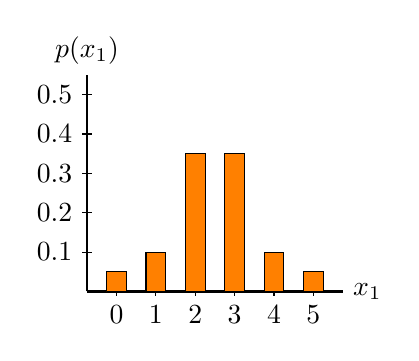
\begin{tikzpicture}
    [scale=0.25]
    %axes
    \draw[thick](0,0)--(0,11) node[above]{$p(x_1)$};
    \draw[thick](0,0)--(13,0) node[right]{$x_1$};
    %label horizontal axis
    \draw (1.5,0.25)--(1.5,-0.25) node[below]{$0$};
    \draw (3.5,0.25)--(3.5,-0.25) node[below]{$1$};
    \draw (5.5,0.25)--(5.5,-0.25) node[below]{$2$};
    \draw (7.5,0.25)--(7.5,-0.25) node[below]{$3$};
    \draw (9.5,0.25)--(9.5,-0.25)
    node[below]{$4$};
    \draw (11.5,0.25)--(11.5,-0.25)
    node[below]{$5$};
    %label vertical axis
    \draw (0.25,2)--(-0.25,2) node[left]{$0.1$};
    \draw (0.25,4)--(-0.25,4) node[left]{$0.2$};
    \draw (0.25,6)--(-0.25,6) node[left]{$0.3$};
    \draw (0.25,8)--(-0.25,8) node[left]{$0.4$};
    \draw (0.25,10)--(-0.25,10) node[left]{$0.5$};
    %histogram
    \draw[fill=orange] (1,0)--(2,0)--(2,1)--(1,1)--(1,0);
    \draw[fill=orange] (3,0)--(3,2)--(4,2)--(4,0)--(3,0);
    \draw[fill=orange] (5,0)--(5,7)--(6,7)--(6,0)--(5,0);
    \draw[fill=orange] (7,0)--(8,0)--(8,7)--(7,7)--(7,0);
    \draw[fill=orange] (9,0)--(10,0)--(10,2)--(9,2)--(9,0);
    \draw[fill=orange]
    (11,0)--(12,0)--(12,1)--(11,1)--(11,0);
    \end{tikzpicture}
&
    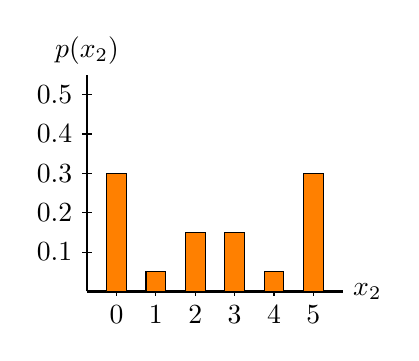
\begin{tikzpicture}
    [scale=0.25]
    %axes
    \draw[thick](0,0)--(0,11) node[above]{$p(x_2)$};
    \draw[thick](0,0)--(13,0) node[right]{$x_2$};
    %label horizontal axis
    \draw (1.5,0.25)--(1.5,-0.25) node[below]{$0$};
    \draw (3.5,0.25)--(3.5,-0.25) node[below]{$1$};
    \draw (5.5,0.25)--(5.5,-0.25) node[below]{$2$};
    \draw (7.5,0.25)--(7.5,-0.25) node[below]{$3$};
    \draw (9.5,0.25)--(9.5,-0.25)
    node[below]{$4$};
    \draw (11.5,0.25)--(11.5,-0.25)
    node[below]{$5$};
    %label vertical axis
    \draw (0.25,2)--(-0.25,2) node[left]{$0.1$};
    \draw (0.25,4)--(-0.25,4) node[left]{$0.2$};
    \draw (0.25,6)--(-0.25,6) node[left]{$0.3$};
    \draw (0.25,8)--(-0.25,8) node[left]{$0.4$};
    \draw (0.25,10)--(-0.25,10) node[left]{$0.5$};
    %histogram
    \draw[fill=orange] (1,0)--(2,0)--(2,6)--(1,6)--(1,0);
    \draw[fill=orange] (3,0)--(3,1)--(4,1)--(4,0)--(3,0);
    \draw[fill=orange] (5,0)--(5,3)--(6,3)--(6,0)--(5,0);
    \draw[fill=orange] (7,0)--(8,0)--(8,3)--(7,3)--(7,0);
    \draw[fill=orange] (9,0)--(10,0)--(10,1)--(9,1)--(9,0);
    \draw[fill=orange]
    (11,0)--(12,0)--(12,6)--(11,6)--(11,0);
    \end{tikzpicture}
&
    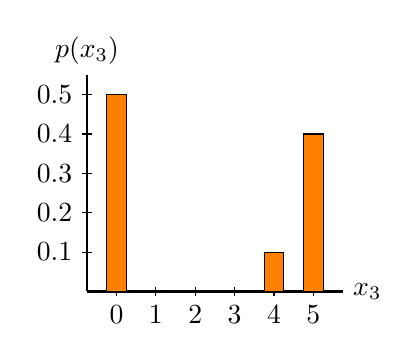
\begin{tikzpicture}
    [scale=0.25]
    %axes
    \draw[thick](0,0)--(0,11) node[above]{$p(x_3)$};
    \draw[thick](0,0)--(13,0) node[right]{$x_3$};
    %label horizontal axis
    \draw (1.5,0.25)--(1.5,-0.25) node[below]{$0$};
    \draw (3.5,0.25)--(3.5,-0.25) node[below]{$1$};
    \draw (5.5,0.25)--(5.5,-0.25) node[below]{$2$};
    \draw (7.5,0.25)--(7.5,-0.25) node[below]{$3$};
    \draw (9.5,0.25)--(9.5,-0.25)
    node[below]{$4$};
    \draw (11.5,0.25)--(11.5,-0.25)
    node[below]{$5$};
    %label vertical axis
    \draw (0.25,2)--(-0.25,2) node[left]{$0.1$};
    \draw (0.25,4)--(-0.25,4) node[left]{$0.2$};
    \draw (0.25,6)--(-0.25,6) node[left]{$0.3$};
    \draw (0.25,8)--(-0.25,8) node[left]{$0.4$};
    \draw (0.25,10)--(-0.25,10) node[left]{$0.5$};
    %histogram
    \draw[fill=orange] (1,0)--(2,0)--(2,10)--(1,10)--(1,0);
    \draw[fill=orange] (3,0)--(3,0)--(4,0)--(4,0)--(3,0);
    \draw[fill=orange] (5,0)--(5,0)--(6,0)--(6,0)--(5,0);
    \draw[fill=orange] (7,0)--(8,0)--(8,0)--(7,0)--(7,0);
    \draw[fill=orange] (9,0)--(10,0)--(10,2)--(9,2)--(9,0);
    \draw[fill=orange]
    (11,0)--(12,0)--(12,8)--(11,8)--(11,0);
    \end{tikzpicture}
\end{tabular}
\end{center}

\begin{center}
\begin{tabular}{ c c c }
% [Histograms code here, unchanged]
\end{tabular}
\end{center}

\begin{itemize}
\item[(a)] Before computing anything and basing your answer solely on the PMF above, put the variances of the three random variables in order from least to greatest. Explain your reasoning.

\vfill
\textcolor{blue}{
Looking at the spread of each histogram: $X_1$ is concentrated in the middle, $X_2$ has more extreme values but balanced, $X_3$ has more probability at extremes. Therefore, $Var(X_1) < Var(X_2) < Var(X_3)$.
}

\item[(b)] Sketch an example of a histogram representing the PMF of a random variable $Y$ having {\bf higher} variance than $X_3$. Sketch an example of a histogram representing the PMF of a random variable $Z$ having the same mean as $X_1$ but {\bf lower} variance than $X_1$.\\

\textcolor{blue}{
- For $Y$: push most probability to the extreme ends (0 and 5) with almost nothing in the middle.  
- For $Z$: cluster most probability close to the mean (e.g., around $x=2$ and $x=3$) and reduce tails.
}
\begin{center}
\begin{tabular}{cc}
    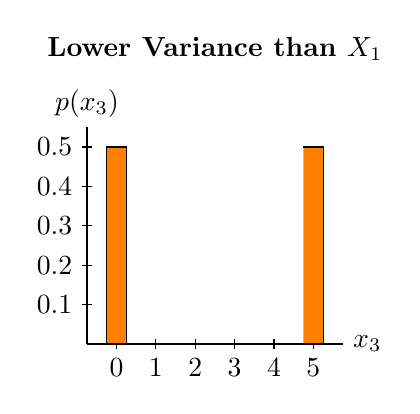
\begin{tikzpicture}
    [scale=0.25]
    % Title
    \node at (6.5, 15) {\textbf{Lower Variance than $X_1$}};
    %axes
    \draw[thick](0,0)--(0,11) node[above]{$p(x_3)$};
    \draw[thick](0,0)--(13,0) node[right]{$x_3$};
    %label horizontal axis
    \draw (1.5,0.25)--(1.5,-0.25) node[below]{$0$};
    \draw (3.5,0.25)--(3.5,-0.25) node[below]{$1$};
    \draw (5.5,0.25)--(5.5,-0.25) node[below]{$2$};
    \draw (7.5,0.25)--(7.5,-0.25) node[below]{$3$};
    \draw (9.5,0.25)--(9.5,-0.25)
    node[below]{$4$};
    \draw (11.5,0.25)--(11.5,-0.25)
    node[below]{$5$};
    %label vertical axis
    \draw (0.25,2)--(-0.25,2) node[left]{$0.1$};
    \draw (0.25,4)--(-0.25,4) node[left]{$0.2$};
    \draw (0.25,6)--(-0.25,6) node[left]{$0.3$};
    \draw (0.25,8)--(-0.25,8) node[left]{$0.4$};
    \draw (0.25,10)--(-0.25,10) node[left]{$0.5$};
    %histogram
    \draw[fill=orange] (1,0)--(2,0)--(2,10)--(1,10)--(1,0);
    % \draw[fill=orange] (3,0)--(3,0)--(4,0)--(4,0)--(3,0);
    % \draw[fill=orange] (5,0)--(5,0)--(6,0)--(6,0)--(5,0);
    % \draw[fill=orange] (7,0)--(8,0)--(8,0)--(7,0)--(7,0);
    % \draw[fill=orange] (9,0)--(10,0)--(10,2)--(9,2)--(9,0);
    \draw[fill=orange]
    (11,0)--(12,0)--(12,10)--(11,10)--(11,10);
    \end{tikzpicture}
&
    \begin{tikzpicture}
    [scale=0.25]
    \node at (6.5, 15) {\textbf{Higher Variance than $X_3$}};

    %axes
    \draw[thick](0,0)--(0,11) node[above]{$p(x_3)$};
    \draw[thick](0,0)--(13,0) node[right]{$x_3$};
    %label horizontal axis
    \draw (1.5,0.25)--(1.5,-0.25) node[below]{$0$};
    \draw (3.5,0.25)--(3.5,-0.25) node[below]{$1$};
    \draw (5.5,0.25)--(5.5,-0.25) node[below]{$2$};
    \draw (7.5,0.25)--(7.5,-0.25) node[below]{$3$};
    \draw (9.5,0.25)--(9.5,-0.25)
    node[below]{$4$};
    \draw (11.5,0.25)--(11.5,-0.25)
    node[below]{$5$};
    %label vertical axis
    \draw (0.25,2)--(-0.25,2) node[left]{$0.1$};
    \draw (0.25,4)--(-0.25,4) node[left]{$0.2$};
    \draw (0.25,6)--(-0.25,6) node[left]{$0.3$};
    \draw (0.25,8)--(-0.25,8) node[left]{$0.4$};
    \draw (0.25,10)--(-0.25,10) node[left]{$0.5$};
    %histogram
    % \draw[fill=orange] (1,0)--(2,0)--(2,10)--(1,10)--(1,0);
    % \draw[fill=orange] (3,0)--(3,0)--(4,0)--(4,0)--(3,0);
    \draw[fill=orange] (5,0)--(6,0)--(6,10)--(5,10)--(5,0);
    \draw[fill=orange] (7,0)--(8,0)--(8,10)--(7,10)--(7,0);
    % \draw[fill=orange] (9,0)--(10,0)--(10,2)--(9,2)--(9,0);
    \draw[fill=orange]
    % (11,0)--(12,0)--(12,10)--(11,10)--(11,10);
    \end{tikzpicture}
\end{tabular}
\end{center}
\hrulefill\\

\begin{center}
({\it Expectation \& Variance of Continuous Random Variables})
\end{center}

\,\hfill \fbox{$\mu=E[X] = \displaystyle\int_{S_X} x\cdot p(x)\,dx$} \hfill\,

\,\hfill \fbox{$Var(X) = E[X^2]-\mu^2=\displaystyle\int_{S_X} x^2\cdot p(x)\,dx-\mu^2$}\hfill\,

\exercise\ltrm{\bf\color{Orange}P2} Let the continuous random variable $V$ have the following PDF:
\[
p(v) = 
\begin{cases} 
\frac{1}{v} & \text{for } 1 \leq v \leq e, \\
0 & \text{otherwise}.
\end{cases}
\]

\begin{itemize}
\item[(a)] Find the mean of $V$.
\textcolor{blue}{
$\displaystyle \mu = \int_1^e v \cdot \frac{1}{v} \, dv = \int_1^e 1\,dv = v\Big|_1^e = e-1 \approx 1.718$
}
    \vfill

\item[(b)] Find the variance of $V$.\\
\textcolor{blue}{
\begin{align*}
E[V^2] &= \int_1^e v^2 \cdot \frac{1}{v} \, dv\\
&= \int_1^e v\, dv = \frac{v^2}{2}\Big|_1^e \\
&= \frac{e^2 - 1}{2} \approx 3.194\\
Var(V) &= E[V^2] - \mu^2 \\
&= \frac{e^2 - 1}{2} - (e-1)^2\\
&= 3.194 - (1.718)^2 \approx 3.194 - 2.95 = 0.244
\end{align*}
}
    \vfill

\end{itemize}

\exercise\ltrm{\bf\color{Orange}P2} The integral $\dint_1^{c} \frac12z\,dz$ represents the expected value of a random variable $Z$, where $c$ is a constant to be determined.\\
\begin{itemize}
\item[(a)] Find the PDF of $Z$.
\textcolor{blue}{
$E[Z] = \int_1^{c} z p(z)\,dz = \int_1^{c} \frac12z\,dz$. So, 
\[
p(z) =
\begin{cases}
 \frac12  & \text{ if } 1 \le z \le c\\
 0 & \text{ otherwise}
\end{cases}
\]
}


\vfill

\item[(b)] Find the value of $c$.\\
\textcolor{blue}{
Solve $\int_1^c \frac12 dz = 1$ (total probability), then 
\begin{align*}
1 &= \int_1^c \frac12 dz = \frac{z}{2}\Big|_1^c \\
&= \frac{c}{4} - \frac12\\
\frac32 &= \frac12 c\\
&\implies c = 3
\end{align*}
}
\vfill

\item[(c)] Find the variance of $Z$.\\
\textcolor{blue}{
$E[Z] = \int_1^{\sqrt{5}} z \cdot \frac12 z dz = \int_1^{\sqrt{5}} \frac{z^2}{2} dz = \frac{1}{6}(z^3)|_1^{\sqrt{5}} = \frac{5\sqrt{5}-1}{6} \approx 1.706$
\begin{align*}
E[Z] &= \int_1^{3} z \cdot \frac12  dz\\
&= \frac{1}{4}z^2|_1^{3}\\
&= \frac94 - \frac14\\
&=2
\end{align*}
\begin{align*}
E[Z^2] &= \int_1^{3} \frac12 \cdot z^2 \ dz\\
&= \frac{1}{6} z^3|_1^{3}\\
&= \frac{27}{6} - \frac16\\
&= \frac{13}{3}
\end{align*}
\begin{align*}
Var(Z) &= E[Z^2] - E[Z]^2 \\
&= \left(\frac{13}{3}\right)^2 - 4^2\\
&= \frac13
\end{align*}
}
\end{itemize}

\newpage
{\bf\color{blue}Extra Practice 1.}\ltrm{{\bf\color{Orange}P1}}
Let $X$ be a discrete random variable with the following probability mass function $p(x)$.

\begin{table}[h!]
        \centering
        \begin{tabular}{c|ccccc}
            \hline
           $x$  & 1 & 2 & 3 & 4 & 5\\
           \hline\\
           $p(x)$  & $\dfrac{3}{10}$ & $\dfrac{1}{10}$ & $\dfrac{1}{10}$ & & $\dfrac{3}{10}$\\\\
           \hline
        \end{tabular}
    \end{table}

\begin{enumerate}
    \item[(a)] Find the missing value in the table so that $p(x)$ is a valid probability mass function.

    {\color{blue}{
    Since this is a probability mass function, the total probability must sum to 1:
    \[
    \frac{3}{10} + \frac{1}{10} + \frac{1}{10} + p(4) + \frac{3}{10} = 1.
    \]
    Summing the known values:
    \[
    \frac{3+1+1+3}{10} = \frac{8}{10}.
    \]
    Therefore,
    \[
    \frac{8}{10} + p(4) = 1 \implies p(4) = \frac{2}{10} = \frac{1}{5}.\]
    }

   {\color{black} \item[(b)] Find the expected value of $X$.}

    \textcolor{blue}{
    The expected value is:
    \[
    E[X] = \sum x p(x).
    \]
    Substitute values:
    \[
    E[X] = 1\cdot\frac{3}{10} + 2\cdot\frac{1}{10} + 3\cdot\frac{1}{10} + 4\cdot\frac{2}{10} + 5\cdot\frac{3}{10}.
    \]
    Compute:
    \[
    = \frac{3}{10} + \frac{2}{10} + \frac{3}{10} + \frac{8}{10} + \frac{15}{10}
    = \frac{31}{10} = 3.1.
    \]
    }

    \vfill

   {\color{black} \item[(c)] Find the variance of $x$.}
    
    \textcolor{blue}{
    First compute $E[X^2]$:
    \[
    E[X^2] = \sum x^2 p(x)
    = 1^2\cdot\frac{3}{10} + 2^2\cdot\frac{1}{10} + 3^2\cdot\frac{1}{10} + 4^2\cdot\frac{2}{10} + 5^2\cdot\frac{3}{10}.
    \]
    \[
    = \frac{3}{10} + \frac{4}{10} + \frac{9}{10} + \frac{32}{10} + \frac{75}{10}
    = \frac{123}{10}.
    \]
    Then:
    \[
    \text{Var}(X) = E[X^2] - (E[X])^2 = \frac{123}{10} - \left(\frac{31}{10}\right)^2.
    \]
    \[
    = \frac{69}{100}  = 0.69
    \]
    }
    
    \vfill
\end{enumerate}

%%%%%%%%%
\newpage%
%%%%%%%%%

{\bf\color{blue}Extra Practice 2.}\ltrm{{\bf\color{Orange}P2}}
Compute the expectation of a continuous random variable $W$ with PDF given by:
\[
p(w) = 
\begin{cases} 
2\sqrt{w} & \text{for } 0 \leq w \leq 1, \\
0 & \text{otherwise}.
\end{cases}
\]

\textcolor{blue}{
The expectation is:
\[
E[W] = \int_0^1 w \cdot 2\sqrt{w}\, dw = \int_0^1 2 w^{3/2} \, dw.
\]
Compute:
\[
= 2 \cdot \frac{w^{5/2}}{5/2} \Big|_0^1 = 2 \cdot \frac{2}{5} = \frac{4}{5}.
\]
}

\vfill

{\bf\color{blue}Extra Practice 3.}\ltrm{{\bf\color{Orange}P2}} 
Let $X$ be a continuous random variable with the following PDF:
\[
p(x) = \frac{1}{x \ln(10)} \quad \text{for } 1 \leq x \leq 10, \quad \text{and } 0 \text{ otherwise}.
\]
\begin{itemize}
    \item[(a)] Compute the expectation $\mu=E[X]$.

    \textcolor{blue}{
    \[
    E[X] = \int_1^{10} x \cdot \frac{1}{x\ln(10)} dx = \frac{1}{\ln(10)} \int_1^{10} 1 \, dx.
    \]
    \[
    = \frac{1}{\ln(10)} (10 - 1) = \frac{9}{\ln(10)}.
    \]
    }

        \vfill
    \item[(b)] Determine the variance $\text{Var}(X)$. You may leave your answer in terms of $\mu$.

    \textcolor{blue}{
    First compute:
    \[
    E[X^2] = \int_1^{10} x^2 \cdot \frac{1}{x\ln(10)} dx = \frac{1}{\ln(10)} \int_1^{10} x \, dx.
    \]
    \[
    = \frac{1}{\ln(10)} \cdot \frac{x^2}{2} \Big|_1^{10}
    = \frac{1}{\ln(10)} \cdot \frac{100 - 1}{2}
    = \frac{99}{2\ln(10)}.
    \]
    Then:
    \[
    \text{Var}(X) = E[X^2] - (E[X])^2
    = \frac{99}{2\ln(10)} - \mu^2 = \frac{99}{2\ln(10)} - \left(\frac{9}{\ln(10)} \right)^2 = \frac{99}{2\ln(10)} - \frac{81}{(\ln(10))^2} 
    \]
    }

        \vfill
        \vfill
\end{itemize}

\end{document}
%%%%%%%%%%%% END DOCUMENT %%%%%%%%%%%%%%%

